\section{Introducción}

\begin{frame}{Automatas Celulares}
    \begin{block}{Son arreglos regulares de celdas individuales de la misma clase.}
    \textbf{Caracteristicas}:
        \begin{itemize}
            \item Finitos estados y discretos.
            \item Estados: Actualizan simultáneamente.
            \item Reglas de actualización determinísticas y uniformes.
            \item Solo se considera un vecindario local.
        \end{itemize}
    \end{block}

    \begin{multicols}{2}
        {Estados: $a_{i}^{(t)}$ $\rightarrow$ Celda $i$ en tiempo $t$}

        {Regla de evolución: $a_{i}^{(t)} = f \left[ \sum_{j=-r}^{j=r}  \alpha_{j} a_{i+j}^{(t-1)} \right]$}
    \end{multicols}
\end{frame}

\begin{frame}{Vecindario}
    \begin{block}{Von Neumann:}
        \begin{minipage}[t]{0.8\linewidth}
            \begin{itemize}
                \item \textbf{2D}: $N_{i,j}^{(vN)}:=\{(a,b) \in L\ |\ |a - i| + |b - j| \leq r\}$.
                \item \textbf{3D}: $N_{i,j, k}^{(vN)}:=\{(a,b,c) \in L\ |\ |a-i| + |b - j| + |c + k| \leq r\}$.
            \end{itemize}
        \end{minipage}%
        \hfill%
        \begin{minipage}[t]{0.2\linewidth}
            \begin{figure}[H]
                \centering
                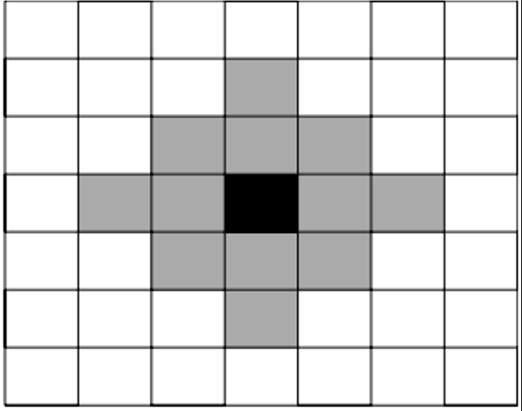
\includegraphics[width=0.7\linewidth]{pic/01-intro/vn}
            \end{figure}
        \end{minipage}

    \end{block}
    \begin{block}{Moore:}
        \begin{minipage}[t]{0.8\linewidth}
            \begin{itemize}
                \item \textbf{2D}: $N_{i,j}^{(M)}:=\{(a,b) \in L\ |\ |a-i|\leq r\ and\ |b - j| \leq r \}$
                \item \textbf{3D}: $N_{i,j,k}^{(M)}:=\{(a, b, c) \in L\ |\ |a-i|\leq r\ and\ |b - j|  \leq r\ and\ |c - k|  \leq r\}$
            \end{itemize}
        \end{minipage}%
        \hfill%
        \begin{minipage}[t]{0.2\linewidth}
            \begin{figure}[H]
                \centering
                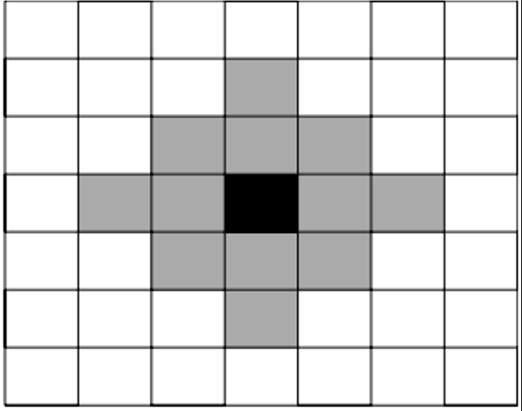
\includegraphics[width=0.7\linewidth]{pic/01-intro/moore}
            \end{figure}
        \end{minipage}

    \end{block}
\end{frame}

\begin{frame}{Game of Life}
    \begin{block}{Reglas:}
        \begin{itemize}
            \item Vecindad de Moore de rango 1 $\longrightarrow$ 8 vecinos.
            \item Dos estados posibles “Viva” o “Muerta” (k = 2).
            \item Celdas Vivas permanecerán vivas si tiene 2 o 3 vecinos vivos, si no muere.
            \item Celdas Muertas se transformarán en Vivas si tiene  3 vecinos vivos.
        \end{itemize}
        \begin{figure}[H]
            \centering
            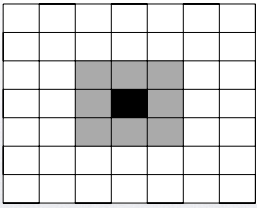
\includegraphics[width=0.2\linewidth]{pic/01-intro/moore_1}
        \end{figure}
    \end{block}
\end{frame}
